\documentclass[runningheads]{llncs}
\usepackage[T1]{fontenc}
\usepackage{amsmath,graphicx,booktabs}
\usepackage[hidelinks]{hyperref}
\newcommand{\pending}[1]{\par\noindent\textbf{Pending:} #1\par}
\begin{document}
\title{AIC26 at VBS 2027: Progressive Hint Memory for Interactive Video Search}
\titlerunning{AIC26: Progressive Hint Memory}
\author{Author list pending}
\institute{Affiliations pending}
\maketitle
\begin{abstract}
Progressively revealed descriptions require an interactive video search system
to retain earlier evidence while allowing new candidates to emerge. We describe
a training-free Progressive Hint Memory (PHM) extension to AIC26. The system
combines video-level evidence from independent hints with a current cumulative
query, and performs bounded in-video retrieval for surviving candidates and new
arrivals. Raw similarities are pooled only within the same model and query before
rank fusion. The interface exposes hint-level evidence and its temporal location
for operator verification. The current implementation has been exercised with
correctness tests and a PE-only live integration smoke test on InfoShot++.
Effectiveness evaluation and competition deployment verification remain pending;
this draft makes no claim of retrieval improvement.
\keywords{Interactive video retrieval \and Progressive descriptions \and Evidence memory}
\end{abstract}

\noindent\textbf{Development draft. Not submission-ready.}
Results, author information, citations and competition deployment coverage
must be completed and independently checked before submission.

\section{Problem and Research Question}
A textual known-item search task may reveal additional details over several
turns. Replacing the query with each new hint can lose earlier evidence; repeatedly
searching the cumulative description provides context but does not explicitly
retain candidate-level observations. Our research question is whether a bounded
memory of evidence and additional in-video retrieval improve prefix video ranking
over cumulative search and fusion of independent hints, when retrievers and
retrieval costs are controlled.

Stateful retrieval, relevance feedback, rank fusion and in-video search have
precedents. Our proposed contribution is their concrete integration for revealed
hints with provenance, bounded candidate retention and consistent local/global
score pooling. Neither reciprocal rank fusion nor geometric averaging is claimed
as a new primitive. \pending{Complete related work, including conversational
Exquisitor, its VBS 2026 in-video search, Robust Relevance Feedback (ICMR 2025),
and query performance prediction. Do not treat their trained feedback gains as
evidence that PHM will achieve comparable gains.}

\section{System and Interaction}
AIC26 provides visual retrieval with PE and, for the supported InfoShot++ profile,
Qwen embeddings; OCR, speech and audio provide optional additional channels.
PHM reuses the internal retrieval service while preserving per-model raw hits,
queries and status before fusion and video grouping. The algorithm configuration
disables query expansion, reranking and TARA. Hybrid channels are an optional
system configuration, separate from the primary visual-only comparison.

A search session represents one target and contains an editable hint ledger.
Each retrieval revision owns its result; only the current revision may commit.
Sessions are isolated between tabs and expire after 60 minutes of inactivity in
a single backend process. A JSONL journal records configuration, released inputs,
retrieval traces and committed snapshots. This journal supports read-only event
replay, without restoring sessions after a process restart.

The operator enters a released hint, inspects rank trajectories, and opens a
representative frame on the timeline. Evidence is labelled by hint and by global,
rescue or backfill origin. A video card flags temporally dispersed evidence and
historical moments without current cumulative support. Selection follows frame
identity when ranking changes. Stability indicators are observations, not estimates
of correctness. Submission remains an explicit operator action.

\begin{figure}[t]
\centering
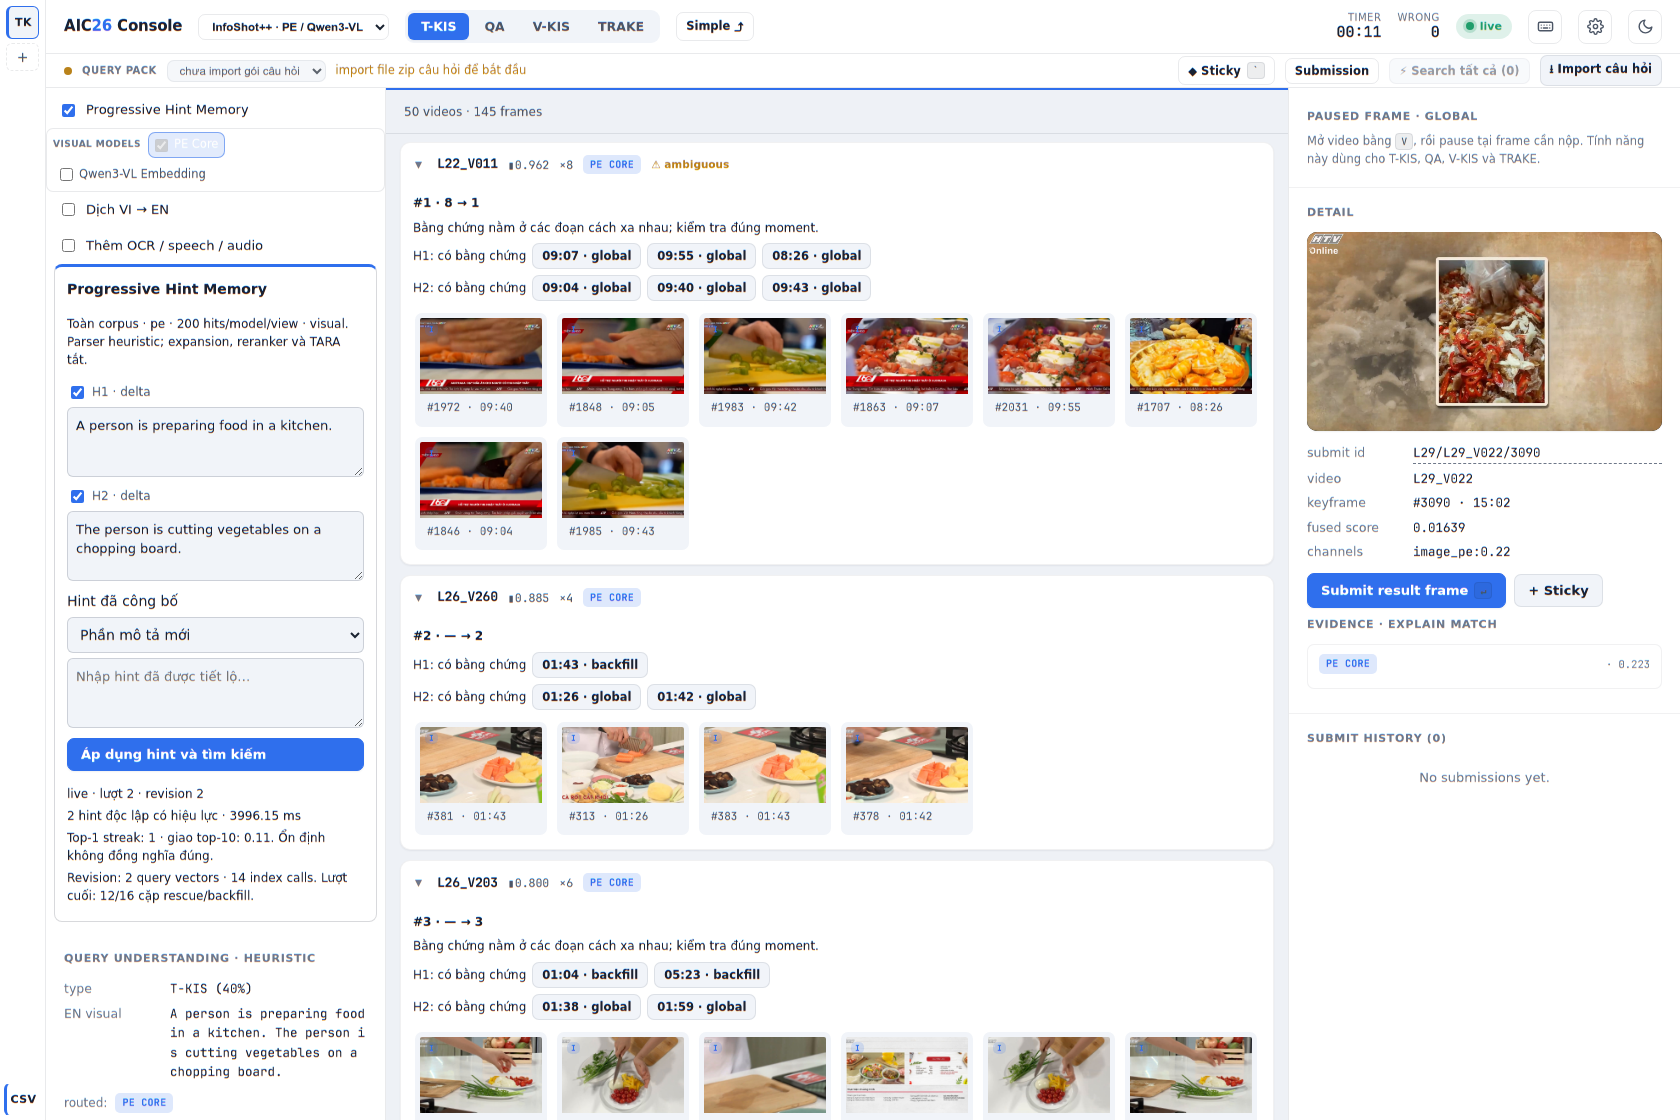
\includegraphics[width=\textwidth]{../../docs/progressive-live-smoke.png}
\caption{PHM in a PE-only live InfoShot++ smoke session with two manually entered
hints. The screenshot illustrates interaction and evidence provenance; this is
not a ground-truth evaluation task.}
\end{figure}
\pending{Finalize an architecture figure and choose a readable crop of the
interaction screenshot after fixing the final paper layout.}

\section{Progressive Hint Memory}
\subsection{Evidence and Scoring}
Unicode and whitespace normalization precede hint processing. A cumulative
description that appends to its predecessor yields one delta hint. Exact repeats
do not add an evidence vote. A cumulative revision that changes previous content
replaces the active description and invalidates derived memory. Retrieval sees
only released and enabled input. Cumulative queries from successive turns are
not counted as independent hints in the memory term.

After within-hint fusion and video grouping, the evidence for video $v$ under
hint $i$ is
\begin{equation}
e_i(v)=\frac{k+1}{k+r_i(v)},\quad k=60,\quad r_i(v)\geq1.
\end{equation}
For an unobserved video, we use $e_i(v)=0$ while retaining an explicit
\emph{unobserved} label. This is a scoring convention for truncated retrieval,
not evidence that the video is irrelevant. Let $I_t$ be the independent hints
with at least one valid channel observation. Memory is
\begin{equation}
M_t(v)=\exp\left(\frac{1}{|I_t|}\sum_{i\in I_t}
\log\left(\epsilon+(1-\epsilon)e_i(v)\right)\right),\quad\epsilon=0.10.
\end{equation}
The cumulative branch at turn $t$ produces rank evidence $C_t(v)$, giving
\begin{equation}
S_t(v)=0.70M_t(v)+0.30C_t(v).
\end{equation}
These are fixed design presets, not calibrated probabilities or optimized
parameters. When delta and cumulative views coincide at the first turn, their
monotonic score transformation preserves the baseline video ordering.

\subsection{Bounded In-Video Retrieval}
After the first turn, up to eight previous candidates missing evidence for the
new hint receive filtered in-video searches. Up to four strong newcomers may
receive backfill searches for previous hints. Allocation is capped at 16
$(\mathrm{video},\mathrm{hint})$ pairs per turn, with up to three frames per
visual model per pair. Encoded query vectors are reused within a session.

Local rank one is not a corpus-wide rank one. Global and local hits for the
same model, query and collection are deduplicated by canonical frame identity,
sorted together by raw similarity, and then assigned candidate-pool ranks for
fusion. Scores from different embedding models are never added. A weak local
hit remains below stronger global hits. Rescue can still promote an incorrect
candidate; its benefit and harm require an ablation.

The ranked memory contains at most 250 videos. Current and previous top-20
candidates are protected, and remaining capacity follows session score with a
stable identifier tie-break. Each hint retains at most three temporally deduplicated
representative frames per video. Backfilled evidence records the turn at which
it was discovered and does not alter earlier committed snapshots.

\section{Evaluation Protocol: Pending Execution}
\pending{No benchmark is run in the current implementation scope. Complete
video-verified annotation using \texttt{TKIS\_queries.xlsx} and the repository's
ground-truth guide before defining an evaluation denominator.}

The intended data consists of synthetic progressive descriptions derived from
existing AIC queries and checked against source video. Ground truth must separate
video identity from valid answer moments; absolute frame indices and keyframe
ordinals must not be confused. Annotation should use verified timestamps and
allow multiple disjoint answer intervals. Duplicate targets and paraphrases must
remain in the same development/evaluation group.

The intended comparisons are cumulative query search, latest-hint search,
Hint-RRF, PHM without rescue/backfill, full PHM, arithmetic memory aggregation,
and a deeper cumulative retrieval control. PE-only precedes PE+Qwen. The planned
primary metric is mean prefix video MRR, averaged per query before aggregation.
Moment Hit@K is measured on the moments actually displayed, separately from
video-level metrics. Rescue recovery and harmful rescue are both reported.
Latency, timeouts, requested query vectors, index calls and returned frames
accompany quality measurements. Paired uncertainty estimates must respect
target-video groups; prefixes are not independent tasks.

\pending{Lock data, translations, splits and cost control on development data;
run evaluation once the protocol is fixed. Insert reproducible tables, paired
intervals and actual denominators. Do not tune the method on evaluation labels.}

\section{Limitations and Deployment Status}
Correctness tests cover hint deduplication and edits, reveal isolation,
first-turn ordering, pooling across local/global retrieval, late revisions,
failure preservation, provenance and identity-based UI selection. Such tests
do not establish effectiveness, usability or competition readiness. A separate
PE-only InfoShot++ browser smoke test exercised two hints, eight survivor rescue
and four newcomer backfill requests, and verified video seeking to the selected
evidence time. This is an integration check, not an evaluated retrieval task.
Video-wide
evidence may be dispersed across unrelated scenes, and rescue may reinforce a
wrong candidate. The operator must still verify an answer moment.

V3C and the other competition collections require separate media registries,
temporal mappings, index coverage and submission checks. Their full ingestion,
external evaluation, operator study and budgeted inspection are planned work.
No calibrated confidence, learned stopping policy or automatic submission is
part of PHM v1.

\section{Conclusion}
The implemented extension makes per-hint candidate evidence explicit and provides
bounded in-video retrieval with consistent score pooling and inspectable temporal
provenance. Its retrieval benefit remains an empirical question. The final paper
must revise this conclusion and the abstract to match the audited experiments
and deployment actually completed.
\end{document}
